In \citet{p9_paper}, we presented our efforts to replicate the MOC model by \citet{cleggRecalibrationMarsScience2017}.
This effort was motivated by our desire to understand the model and its performance better, and to experiment with its components to determine how it could be improved.
However, as discussed, there were some differences between our replica and the original model.
For example, because \citet{cleggRecalibrationMarsScience2017} did not describe when in the pipeline MAD-based outlier removal was performed, we did not include it in our pipeline and instead dedicated an experiment to figuring out when in the pipeline it had the best effect.
Following these experiments, we have now updated our pipeline to more accurately reflect the original MOC model.
Table \ref{tab:replica_results_rmses} shows the RMSEs of the original models and our replicas after these changes.
Figure~\ref{fig:rmse_histograms} illustrates the distribution of these RMSEs as a grouped histogram.
This replica serves as our baseline for the rest of the paper.


\begin{table*}
\centering
\begin{tabular*}{\textwidth}{@{\extracolsep{\fill}}lllllll}
\hline
Element    & PLS1-SM (original) & PLS1-SM (replica) & ICA (original) & ICA (replica) & MOC (original) & MOC (replica) \\
\hline
\ce{SiO2}  & 4.33               & 4.52              & 8.31           & 8.66          & 5.83           & 5.64
\ce{TiO2}  & 0.94               & 0.50              & 1.44           & 0.54          & 1.10           & 0.48
\ce{Al2O3} & 2.85               & 1.80              & 4.77           & 3.37          & 3.18           & 1.84
\ce{FeO_T} & 2.01               & 1.94              & 5.17           & 2.87          & 2.90           & 1.82
\ce{MgO}   & 1.06               & 0.91              & 4.08           & 3.01          & 2.30           & 1.56
\ce{CaO}   & 2.65               & 1.77              & 3.07           & 3.28          & 1.14           & 2.09
\ce{Na2O}  & 0.62               & 0.82              & 2.29           & 2.11          & 1.34           & 1.34
\ce{K2O}   & 0.72               & 0.73              & 0.98           & 1.37          & 1.49           & 1.16
\hline
\end{tabular*}
\caption{RMSE of the original and our replicas of the PLS1-SM, ICA, and MOC models.}
\label{tab:replica_results_rmses}
\end{table*}

\begin{figure*}[ht]
	\centering
	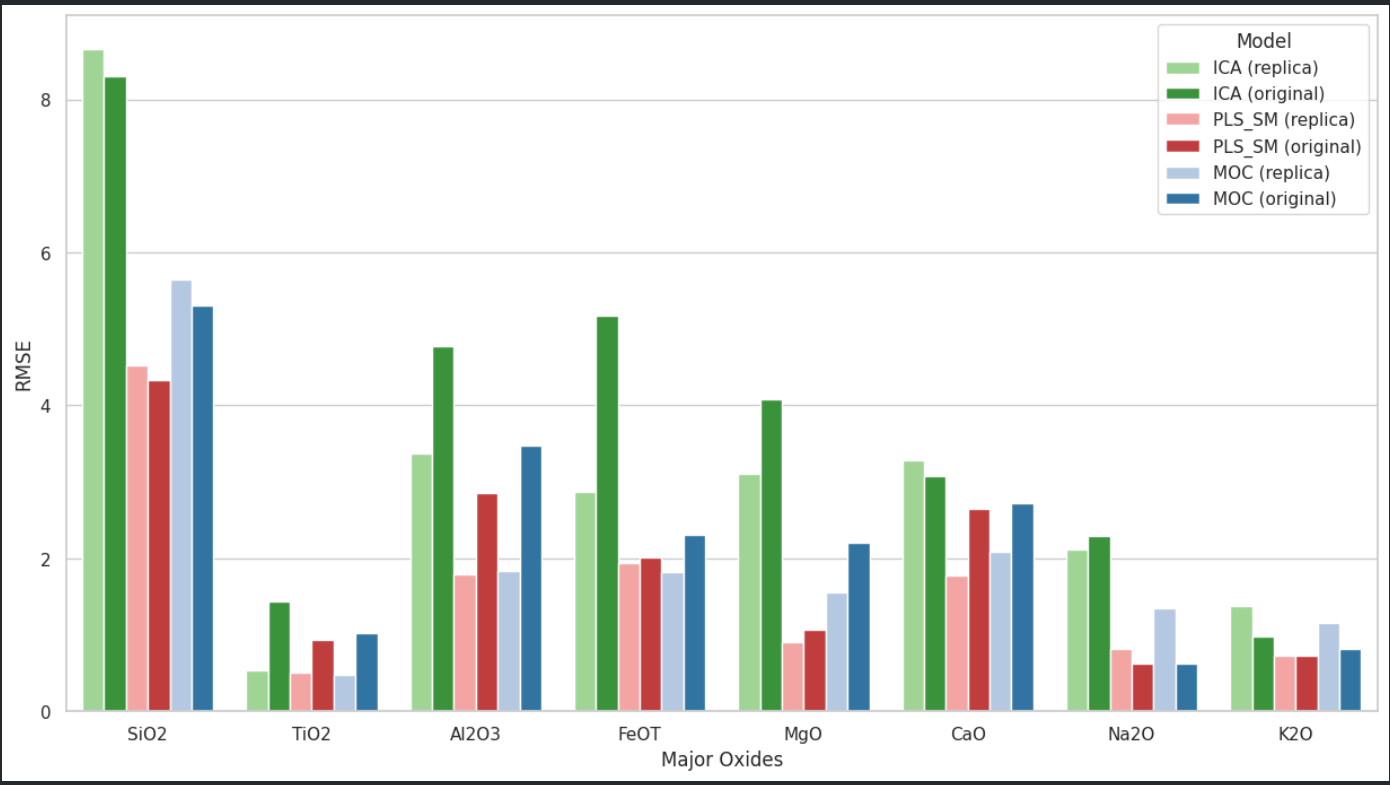
\includegraphics[width=0.85\textwidth]{images/rmse_historgram.png}
	\caption{Grouped histogram of the RMSEs of the original and our replicas of the PLS1-SM, ICA, and MOC models.}
	\label{fig:rmse_histograms}
\end{figure*}

% TODO: Create t-tests and present the results here